\begin{figure}[t!]
\begin{center}
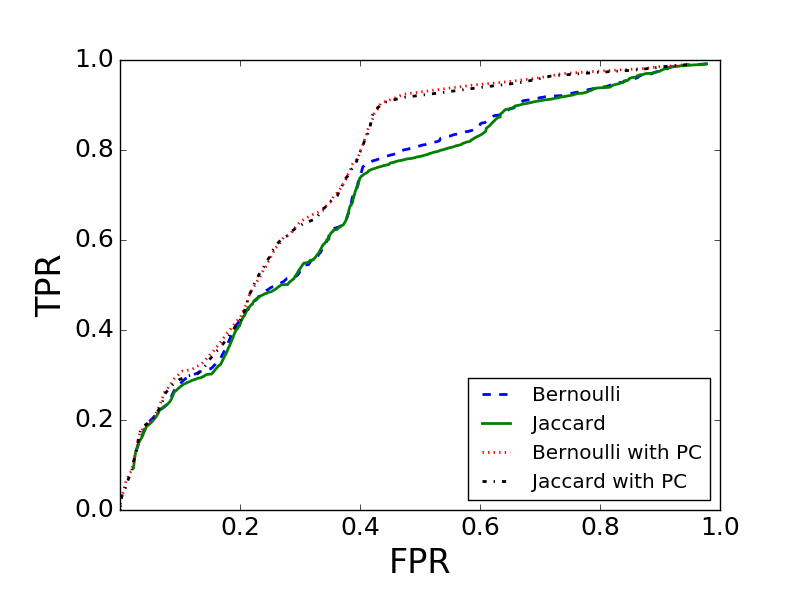
\includegraphics[width=2.5in]{figure/predict}
\mycaption{fig:predict}{ROC comparisons of Static Models.}
{\footnotesize{(How true positive rate (TPR) changes with false positive rate (FPR). 
We change probability threshold from 0.1\% to 99.9\% with step 0.1\%. 
We compute TPR and FPR for each probability threshold to draw the curve.)}}
\end{center}
%\vspace{-0.25in}
\end{figure}